\documentclass[a4paper, 12pt]{article}

\usepackage[portuges]{babel}
\usepackage[utf8]{inputenc}
\usepackage{amsmath, amsthm,amssymb}
\usepackage{indentfirst}
\usepackage{graphicx}
\usepackage{url}
\usepackage{float}
\usepackage{subcaption}

\newtheorem{defin}{Definição}[section]
\newtheorem{obs}{Observação}[section]
\newtheorem{teo}{Teorema}[section]
\newtheorem{nota}{Nota}[section]
\newtheorem{lema}{Lema}[section]



%Python code

\usepackage{listings}
\usepackage{xcolor}
\definecolor{codegreen}{rgb}{0,0.6,0}
\definecolor{codegray}{rgb}{0.5,0.5,0.5}
\definecolor{codepurple}{rgb}{0.58,0,0.82}
\definecolor{backcolour}{rgb}{0.95,0.95,0.92}

\lstdefinestyle{mystyle}{
	backgroundcolor=\color{backcolour},   
	commentstyle=\color{codegreen},
	keywordstyle=\color{magenta},
	numberstyle=\tiny\color{codegray},
	stringstyle=\color{codepurple},
	basicstyle=\ttfamily\footnotesize,
	breakatwhitespace=false,         
	breaklines=true,                 
	captionpos=b,                    
	keepspaces=true,                 
	numbers=left,                    
	numbersep=5pt,                  
	showspaces=false,                
	showstringspaces=false,
	showtabs=false,                  
	tabsize=2
}

\lstset{style=mystyle}


\setlength{\unitlength}{1cm}
\thicklines

\begin{document}

\begin{titlepage}
	\begin{center}
		
		\begin{figure}[!htb]
			\centering
			
\includegraphics[width=5cm]{uminho}
			\label{Rotulo}
		\end{figure}
		%\vspace{1cm}
		
		\textbf{\Huge{Universidade do Minho}}\\
		\vspace{10pt}
		\large{Escola de Ciências da Universidade do Minho}\\
		\large{Departamento de Informática}\\
		\vspace{10pt}
		\normalsize{Mestrado em Matemática e Computação}\\
		\normalsize{Mestrado Integrado em Engenharia Informática}\\
		\vspace{2cm}
		\textbf{\Large{Redes Neuronais Recorrentes para previsão do fluxo de tráfego rodoviário}}\\
		\vspace{2cm}
	\end{center}
	
	\begin{center}
		\textbf{Alunos:}
		\vspace{0,1cm}
		\\Andreia Costa (PG37013) \\Henrique Faria (A82200) \\ Paulo Barbosa (PG40160) \\ Rui Teixeira (PG37021)\\
		\vspace{1cm}
		\textbf{Docentes:} \\
		Bruno Fernandes\\ 
		Victor Alves \\
		\vspace{1cm}
		\textbf{Unidade Curricular:} Classificadores e Sistemas Conexionistas
	\end{center}
	\vspace{1cm}
	\begin{center}
		Maio\\
		2020
	\end{center}
\end{titlepage}

\newpage
% % % % % % % % % % % % % % % % % % % % % % % % % %
\newpage
\tableofcontents
\thispagestyle{empty}

\newpage
\pagenumbering{arabic}

\section{Introdução}


\newpage

\section{\textit{Dataset}}

Aquando da apresentação do presente trabalho foram disponibilizados dados referentes a duas cidades: Braga e Porto, sendo que o grupo escolheu os dados relativos à cidade de Braga para trabalhar.

Os dados encontram-se distribuídos em $4$ \textit{datasets}:

\begin{itemize}
	\item \textit{Traffic Flow Braga Until 20191231};
	\item \textit{Traffic Incidents Braga Until 20191231};
	\item \textit{Weather Braga Descriptions Until 20191231};
	\item \textit{Weather Braga Until 20191231}.
\end{itemize}

Todos os \textit{datasets} contêm dados relativos ao período entre $15$ Janeiro $2019$ e $31$ Dezembro $2019$.

\subsection{\textit{Traffic Flow Braga}}

O \textit{dataset "Traffic Flow Braga" } é constituído pelos seguintes atributos:

\begin{itemize}
	\item $city\_name$;
	\item $road\_num$;
	\item $road\_name$;
	\item $functional\_road\_class\_desc$;
	\item $current\_speed$;
	\item $free\_flow\_speed$;
	\item $speed\_diff$;
	\item $current\_travel\_time$;
	\item $free_flow\_travel\_time$;
	\item $time\_diff$;
	\item $creation\_date$.
\end{itemize}

\subsection{\textit{Traffic Incidents Braga}}

\begin{itemize}
	\item $city\_name$;
	\item $description$;
	\item $cause\_of\_incident$;
	\item $from\_road$;
	\item $to\_road$;
	\item $affected\_roads$;
	\item $incident\_category\_desc$;
	\item $magnitude\_of\_delay\_desc$;
	\item $length\_in\_meters$;
	\item $delay\_in\_seconds$;
	\item $incident\_date$;
	\item $latitude$;
	\item $longitude$.
\end{itemize}

\subsection{\textit{Weather Braga Descriptions}}

\begin{itemize}
	\item $city\_name$;
	\item $cloudiness$;
	\item $atmosphere$;
	\item $snow$;
	\item $thunderstorm$;
	\item $rain$;
	\item $sunrise$;
	\item $sunset$;
	\item $creation\_date$.
\end{itemize}

\subsection{\textit{Weather Braga}}

\begin{itemize}
	\item $city\_name$;
	\item $temperature$;
	\item $atmospheric\_pressure$;
	\item $humidity$;
	\item $wind\_speed$;
	\item $clouds$;
	\item $precipitation$;
	\item $current\_luminosity$;
	\item $sunrise$;
	\item $sunset$;
	\item $creation\_date$.
\end{itemize}

\subsection{Preparação dos dados}
\label{section:falta}

Após análise dos quatro \textit{datasets} concluiu-se que, antes de se desenvolver o modelo para a previsão da \textit{feature speed\_diff}, era necessário fazer uma prévia preparação dos dados.

Começou-se por fazer um tratamento inicial do \textit{dataset Traffic\_Incidents}. Para isso, a cada incidente atribuiu-se os vários valores da coluna \textit{road\_num}, para que posteriormente fosse possível avaliar a distância entre os incidentes e as ruas em estudo e verificar de que forma estes incidentes afetam uma determinada rua.

\begin{figure}[H]
	\centering
	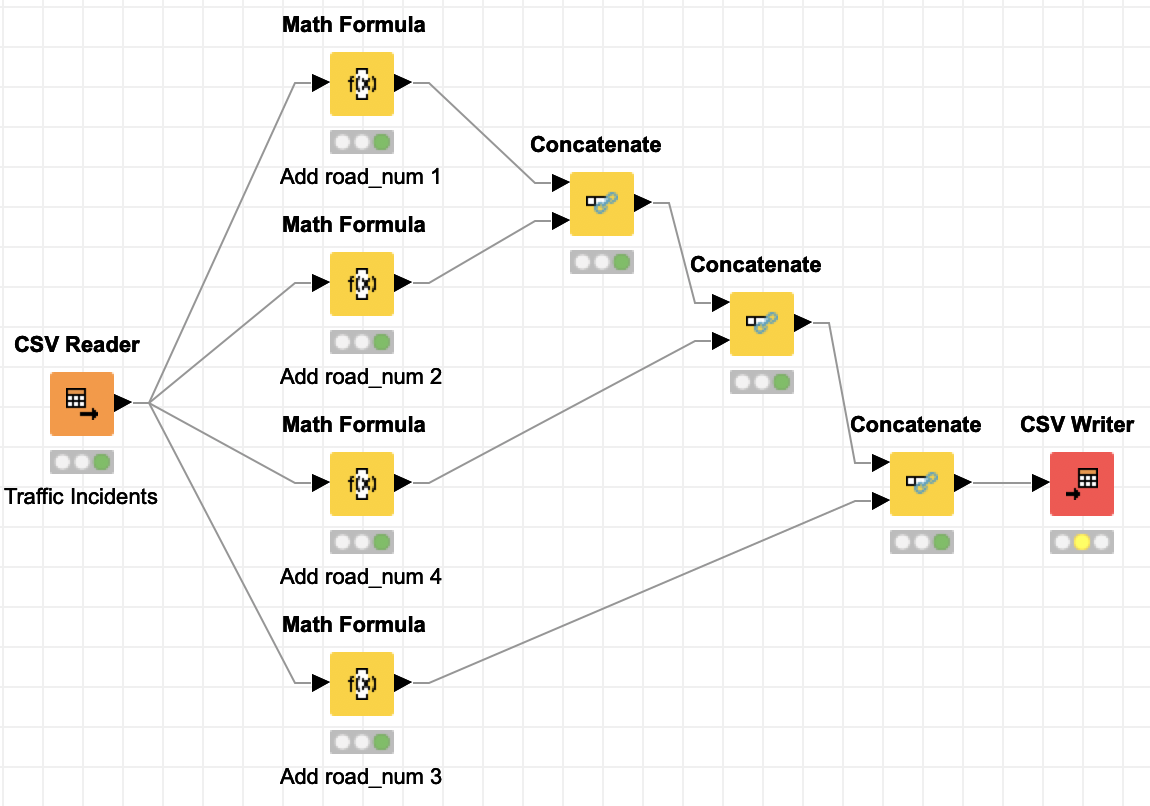
\includegraphics[width=10cm]{Traffic_Incidents}
	\caption{Preparação do \textit{dataset Traffic\_Incidentes}.}
\end{figure}

De seguida, recorrendo à latitude e longitude dos diferentes acontecimentos, calculou-se a distância dos incidentes a cada uma das ruas, para perceber o raio de influência dos incidentes para as ruas em estudo, de modo, a ser possível, posteriormente, remover incidentes que se encontrem muito afastados das ruas em estudo. Para isso, recorreu-se à fórmula:

$$dist(A, B) = R * \arccos (sin (lat_A) * \sin (lat_B) + \cos (lat_A) * \cos (lat_B) * \cos (lon_A-lon_B)). $$

onde,

\begin{itemize}
	\item \textbf{$lat_A$:} latitude do ponto A;
	\item \textbf{$lat_B$:} latitude do ponto B;
	\item \textbf{$lon_A$:} longitude do ponto A;
	\item \textbf{$lon_B$:} longitude do ponto B;
	\item \textbf{$R$:} raio da Terra.
\end{itemize}

tendo-se implementado o seguinte código.

\begin{lstlisting}[language=Python]
import pandas as pd
from math import radians, sin, cos, atan2, sqrt

df = pd.read_csv('Traffic_Incidents.csv', delimiter = ',', error_bad_lines = False, encoding = 'ISO-8859-1')

def distance(p1, n):
	R = 6371.0
	if n == 1:
	lat2 = radians(41.548331)
	lon2 = radians(-8.421298)
	elif n == 2:
	lat2 = radians(41.551356)
	lon2 = radians(-8.420001)
	elif n == 3:
	lat2 = radians(41.546639)
	lon2 = radians(-8.433517)
	else:
	lat2 = radians(41.508849)
	lon2 = radians(-8.462299)
	lat1, lon1 = radians(p1[0]), radians(p1[1])
	dlon = lon2 - lon1
	dlat = lat2 - lat1
	a = sin(dlat / 2)**2 + cos(lat1) * cos(lat2) * sin(dlon / 2)**2
	c = 2 * atan2(sqrt(a), sqrt(1 - a))
	distance = R * c
return distance

df['Distance'] = df.apply(lambda row: distance((row['latitude'],row['longitude']), row['road_num']), axis=1)
\end{lstlisting}

Após calculadas todas as distâncias fez-se um tratamento estatístico, tendo-se obtido os seguintes resultados:

\begin{itemize}
	\item ${max}= 6313,251$;
	\item ${min}= 0,0228$;
	\item ${mean}= 4,507$;
	\item ${standard \ deviation}= 81,789$.
\end{itemize}

Através dos resultados obtidos é possível verificar que existem dados mal classificados, uma vez que, sendo os dados recolhidos referentes apenas à cidade de Braga era impossível que a distância máxima dos incidentes às ruas fosse de cerca de $6313$ km. Fez-se um estudo desta informação e verificou-se que estes dados dizem respeito a uma cidade que não pertence a Braga.

\begin{figure}[H]
	\centering
	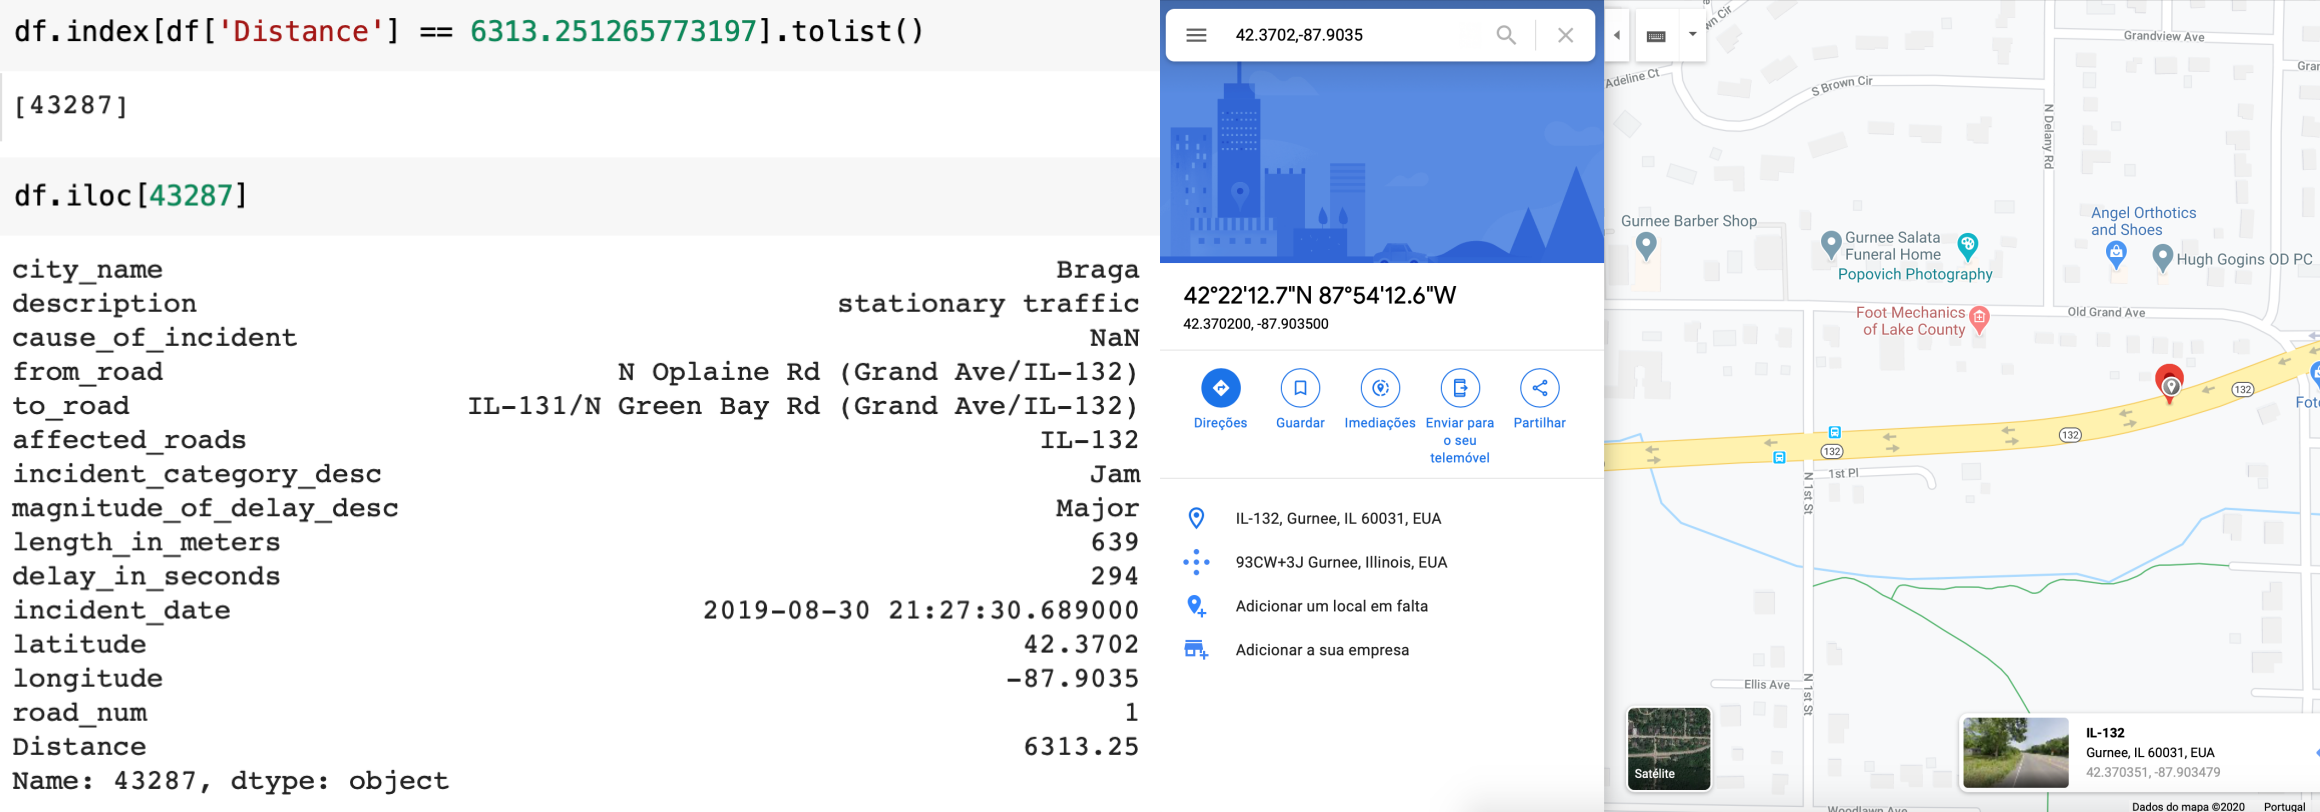
\includegraphics[width=14cm]{EUA}
	\caption{Dado mal classificado.}
\end{figure}

Devido a este facto, optou-se por remover alguns dados do \textit{dataset}. Uma vez que a distância é medida em linha reta utilizou-se como \textit{threshold}, para remover dados, vários valores, nomeadamente, $0.5$, $1$ e $1.5$.

Após feito este tratamento procedeu-se à preparação dos dados referentes aos restantes \textit{datasets}, com o intuito de se obter, no final, um único \textit{dataset}.

Começou-se por fazer o tratamento do \textit{dataset Weather\_Descriptions\_Braga}, tendo-se removido as colunas: \textit{city\_name}, \textit{snow} e \textit{cloudiness}. A coluna \textit{snow} apresentava apenas \textit{missing values}, daí se ter optado pela sua remoção. Relativamente à  coluna \textit{cloudiness}, optou-se por fazer a remoção da mesma, uma vez que existe uma coluna que está diretamente relacionada com esta, a coluna \textit{cloud}, pertencente ao \textit{dataset Weather\_Braga}, e que não apresenta \textit{missing values}.

De seguida, procedeu-se à remoção das colunas \textit{city\_name} e \textit{precipitation} do \textit{dataset Weather\_Braga}. A remoção da coluna \textit{precipitation} deveu-se ao facto desta apenas apresentar um único valor, o $0$. 

De modo a unir o resultado da preparação dos dados feita para os \textit{datasets} anteriores, recorreu-se ao nodo \textit{Joiner}, e uniram-se os \textit{datasets} por \textit{creation\_date}, tendo-se efetuado, de seguida, a extração da data e do tempo, tendo-se extraído: o mês como uma variável numérica, a hora, o dia do mês e o dia da semana.

\begin{figure}[H]
	\centering
	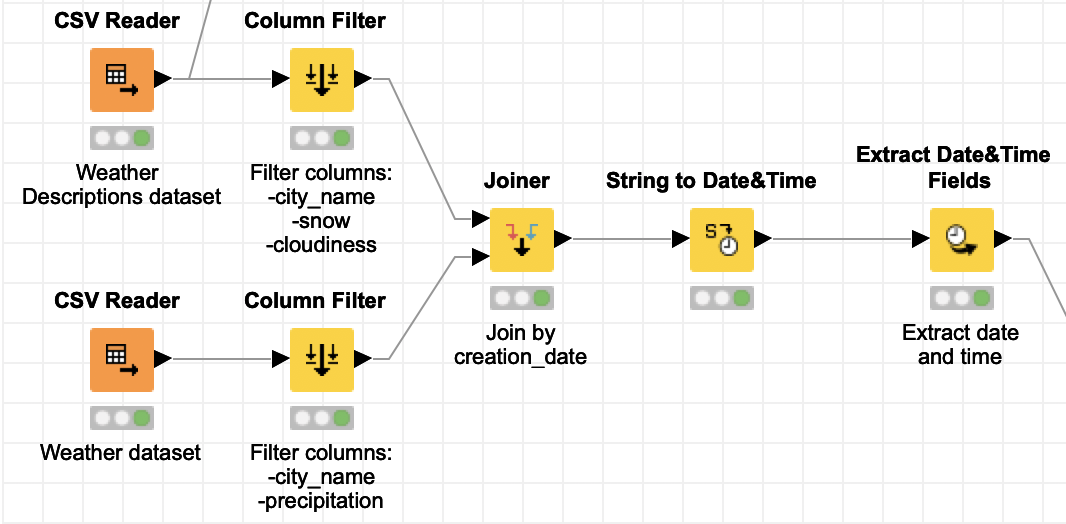
\includegraphics[width=10cm]{weather}
	\caption{Preparação dos \textit{datasets Weather\_Descriptions\_Braga} e \textit{Weather\_Braga}.}
\end{figure}

De seguida, procedeu-se à preparação do \textit{dataset Traffic\_Flow\_Braga}, procedendo-se à remoção das colunas \textit{city\_name} e \textit{road\_name}, seguida da extração da data e hora, à semelhança do que foi feito para o \textit{dataset} anterior.

O \textit{dataset Traffic\_Flow\_Braga} tinha registos de $20$ em $20$ minutos e o \textit{dataset} obtido anteriormente tinha registos de hora em hora, assim, de modo a unir o \textit{dataset} com os dados relativos ao \textit{Weather}, optou-se por agrupar os registos do \textit{dataset Traffic\_Flow\_Braga} por hora, mês, dia e rua, recorrendo-se ao nodo \textit{GroupBy}, tendo-se feito a média de todos os valores numéricos para as restantes colunas.

Assim, de modo a juntar este \textit{dataset} ao obtido anteriormente, recorreu-se ao nodo \textit{Joiner}, unindo-se os \textit{datasets} por hora, dia do mês e mês, fazendo-se um \textit{Left Outer Join}. Optou-se por fazer um \textit{Left Outer Join}, uma vez que não se queriam as condições atmosféricas de registos em que não havia dados de tráfego.

\begin{figure}[H]
	\centering
	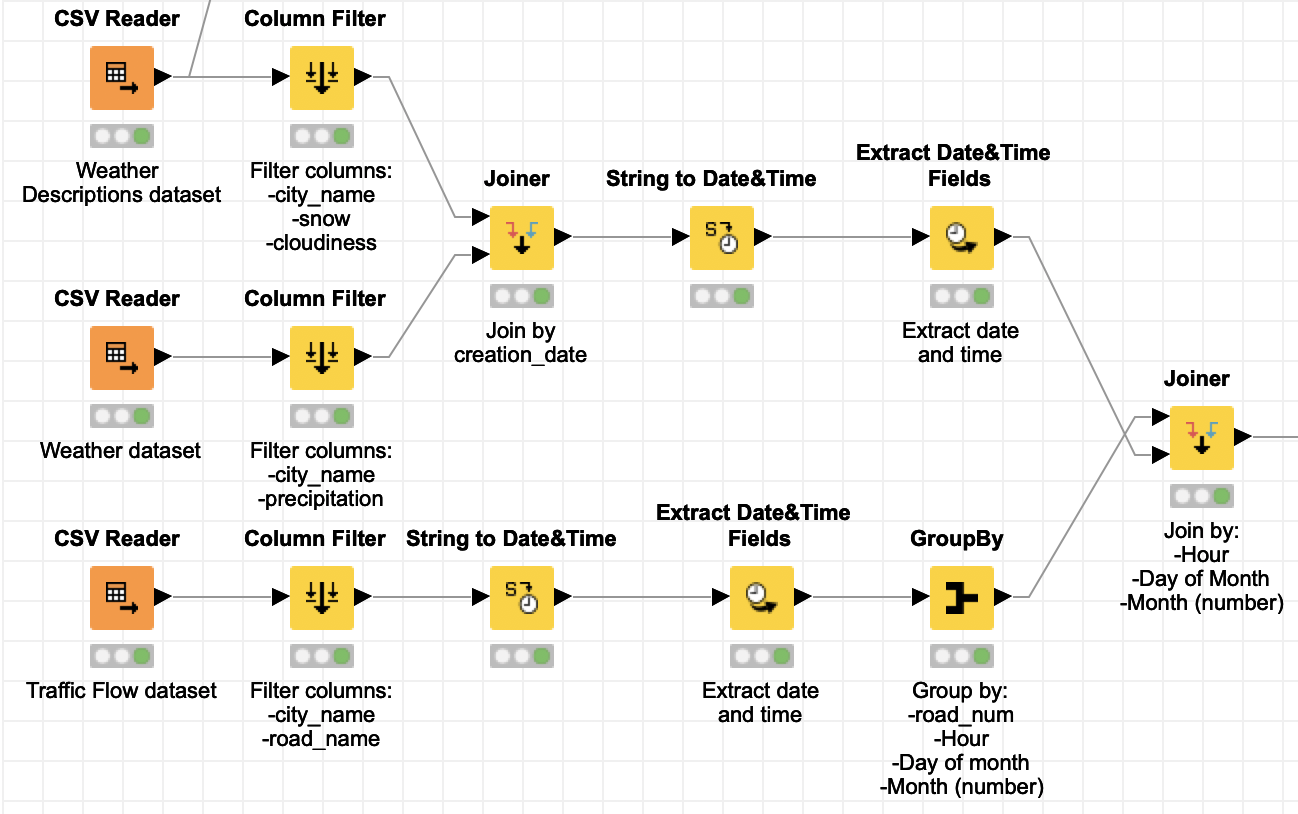
\includegraphics[width=10cm]{join}
	\caption{Preparação do \textit{dataset Traffic\_Flow\_Braga}.}
\end{figure}

Após a junção dos \textit{datasets}, eliminou-se a coluna \textit{creation\_date} e transformaram-se os valores "N/A", das colunas \textit{rain}, \textit{thunderstorm} e \textit{atmosphere}, em \textit{missing values}, recorrendo ao nodo \textit{String Manipulation}. De seguida, quando não existiam valores na coluna \textit{rain} atribuia-se o valor da coluna \textit{thunderstorm}, uma vez que as \textit{labels} da coluna \textit{thunderstorm} faziam referência ao estado da chuva. De seguida, alteraram-se alguns dos valores ($"trovoada \ com \ chuva \ fraca" \rightarrow "chuva \ fraca"$, $"trovoada \ com \ chuva \ forte" \rightarrow "chuva \ forte"$ e $"trovoada" \rightarrow "chuva"$), tendo-se removido, no final, a coluna \textit{thunderstorm}. Por fim, eliminaram-se as colunas \textit{sunrise} e \textit{sunset}, uma vez que não se achou que estas colunas eram relevantes para prever o \textit{speed\_diff}.

\begin{figure}[H]
	\centering
	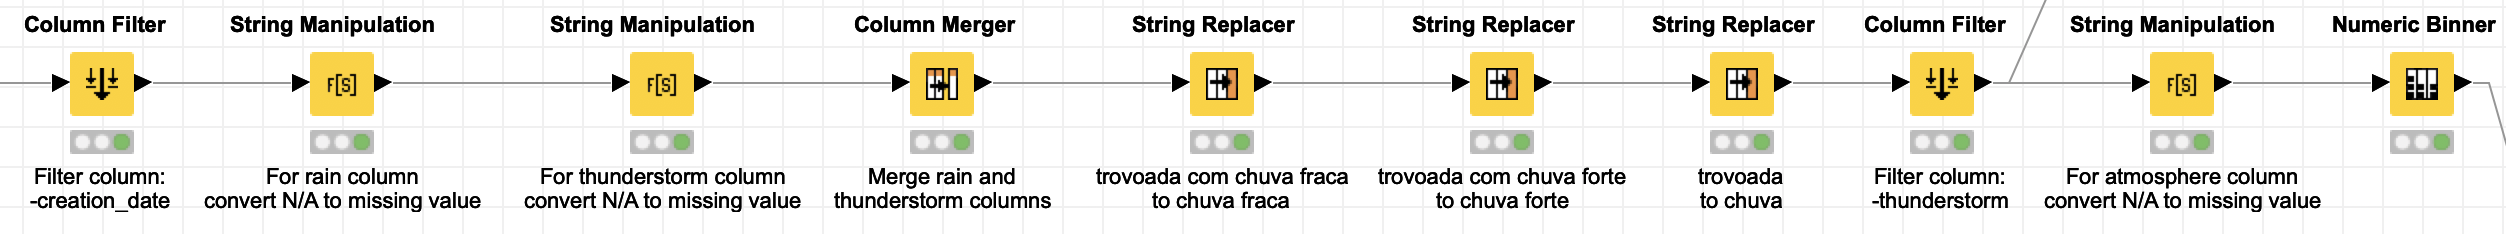
\includegraphics[width=15cm]{prep}
	\caption{Preparação dos dados.}
\end{figure}

Por fim, tratou-se o \textit{dataset Traffic\_Incidents\_Braga} cuja \textit{feature Distance} tinha apenas valores inferiores a $0.5 \ km$. Recorrendo à coluna \textit{incident\_date}, procedeu-se à extração do dia, da hora e do mês e removeram-se colunas irrelevantes, nomeadamente, as colunas \textit{city\_name}, \textit{incident\_date} e \textit{cause\_of\_incident}, uma vez que esta última apresentava maioritariamente \textit{missing values}.

Uma vez que a coluna \textit{Distance} já inclui informação que permite relacionar a influência de um dado inicidente com as ruas em estudo, optou-se por remover as colunas: \textit{from\_road}, \textit{to\_road}, \textit{affected\_roads}, \textit{latitute} e \textit{longitude}.

Após tratado este \textit{dataset}, e recorrendo ao nodo \textit{Joiner}, uniu-se este \textit{dataset} com o obtido anteriormente por hora, dia do mês, mês e \textit{road\_num}. Deste modo, uniram-se os $4$ \textit{datasets} iniciais num único.

\begin{figure}[H]
	\centering
	\includegraphics[width=10cm]{Incident}
	\caption{Preparação do \textit{dataset} resultante do tratamento do \textit{dataset Traffic\_Incidents\_Braga}.}
\end{figure}

Após se ter apenas um \textit{dataset} verificou-se que este continha $26$ colunas, o que se achou serem demasiadas. Assim, de modo a tornar o \textit{dataset} mais pequeno, recorreu-se ao nodo \textit{Rank Correlation} e avaliou-se a correlação que existia entre as diferentes colunas, tendo-se removido as seguintes: \textit{free\_flow\_speed}, \textit{current\_travel\_time}, \textit{free\_flow\_travel\_time }, \textit{atmospheric\_pressure}, \textit{humidity}, \textit{current\_luminosity} e \textit{magnitude\_of\_delay\_desc}. Deste modo, o \textit{dataset} ficou apenas com $18$ colunas.

\begin{figure}[H]
	\centering
	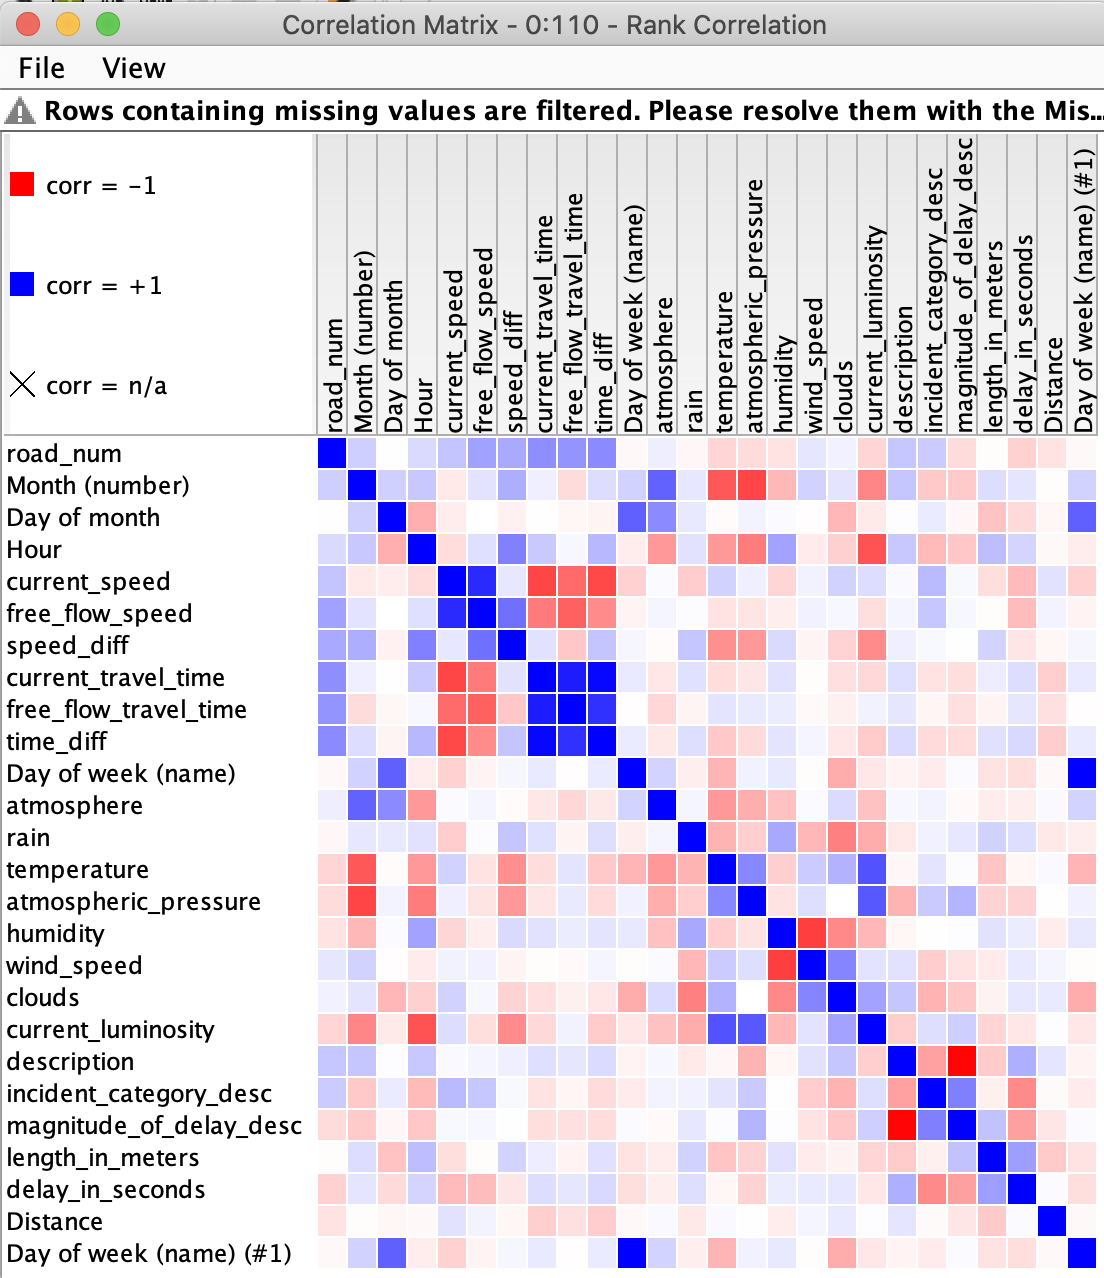
\includegraphics[width=10cm]{rank}
	\caption{Análise da correlação entre as diferentes \textit{features}.}
\end{figure}

Aos valores \textit{Undefined} da \textit{feature descriptions} atribui-se o valor \textit{Unknown Delay}, uma vez que estes têm significado semelhante.

De seguida, e tendo em conta que as colunas \textit{atmosphere} e \textit{rain} apresentam muitos \textit{missing values}, procedeu-se ao tratamento dos mesmos. 

Começou-se, então, por tratar os \textit{missing values} da coluna \textit{atmosphere}, uma vez que esta era a que apresentava menos \textit{missing values}, tendo-se separado o \textit{dataset} em dois, recorrendo ao nodo \textit{Rule-based Row Splitter}. Um \textit{dataset} apresenta a coluna \textit{atmosphere} apenas com \textit{missing values} e o outro apresenta a coluna \textit{atmosphere} com os vários valores. De seguida, utilizaram-se \textit{Random Forest} para fazer a previsão dos \textit{missing values}.

Com o intuito de perceber quais os melhores parâmetros a utilizar efetuou-se o \textit{tunning} do modelo.

\begin{figure}[H]
	\centering
	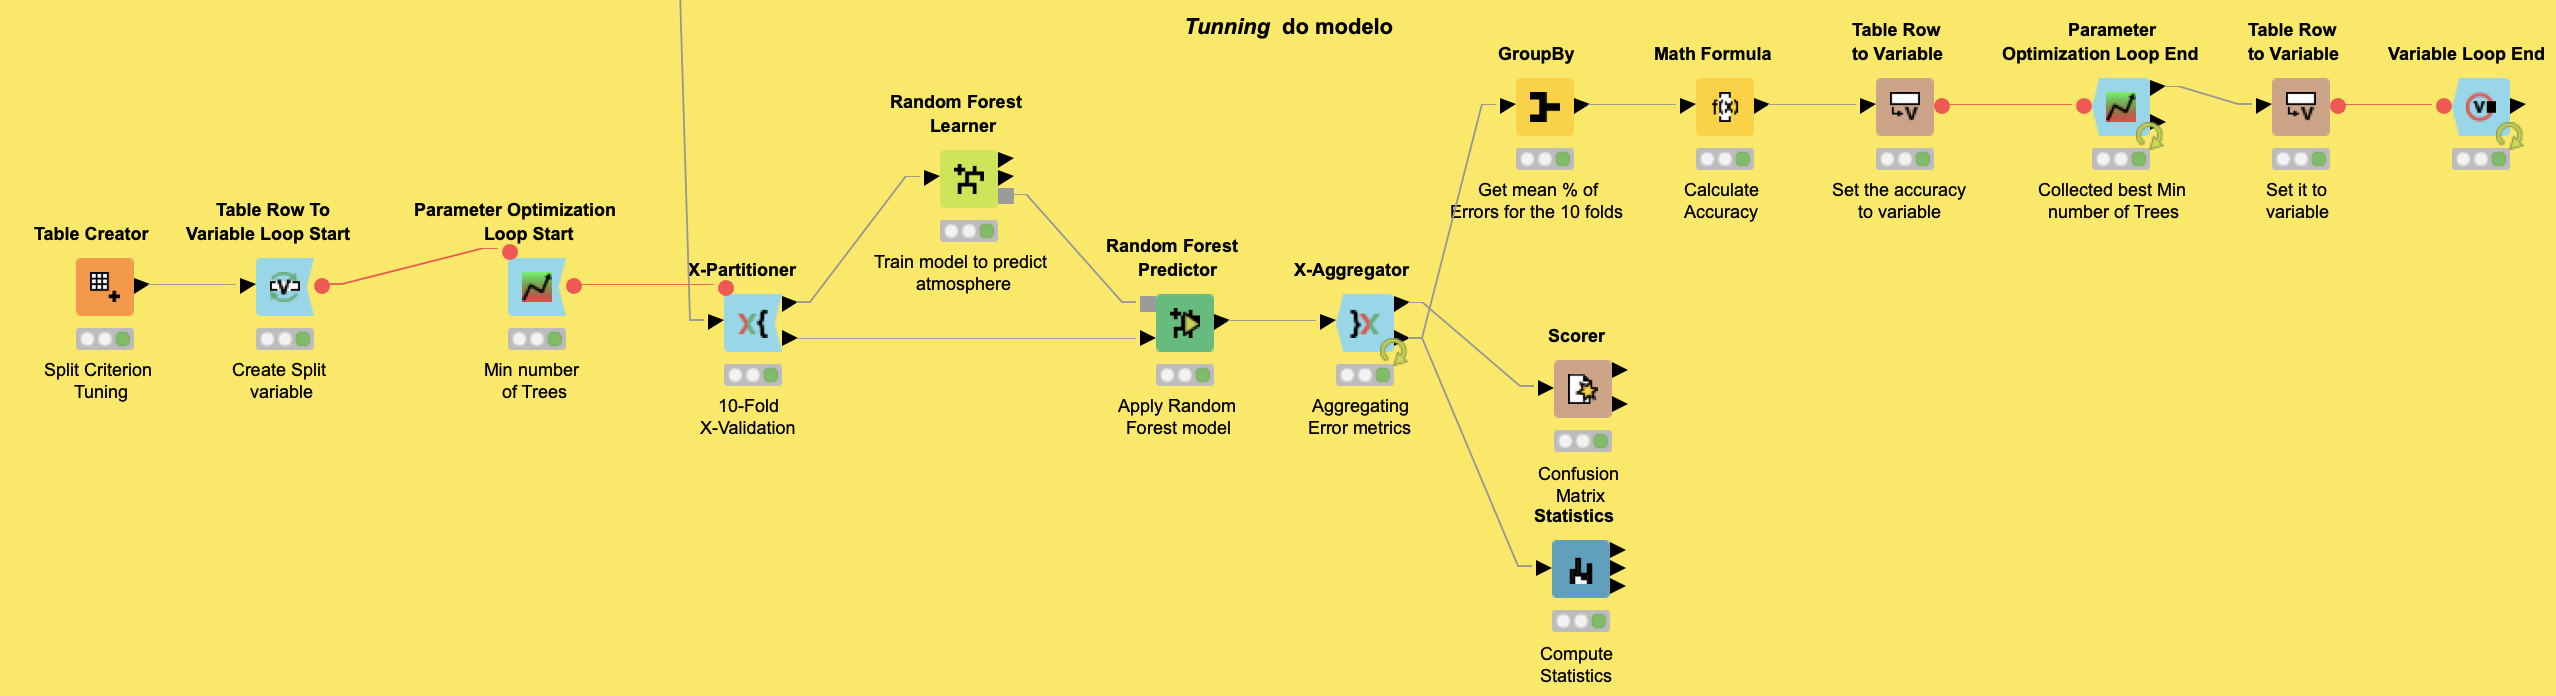
\includegraphics[width=15cm]{tunning}
	\caption{\textit{Tunning} do modelo.}
\end{figure}

Após efetuado o \textit{tunning} do modelo, concluiu-se que este apresentava melhores valores se fosse treinado com $60$ árvores e usando como critério de \textit{split} o \textit{Information Gain}, tendo-se uma \textit{accuracy} de cerca $99,5\%$

\begin{figure}[H]
	\centering
	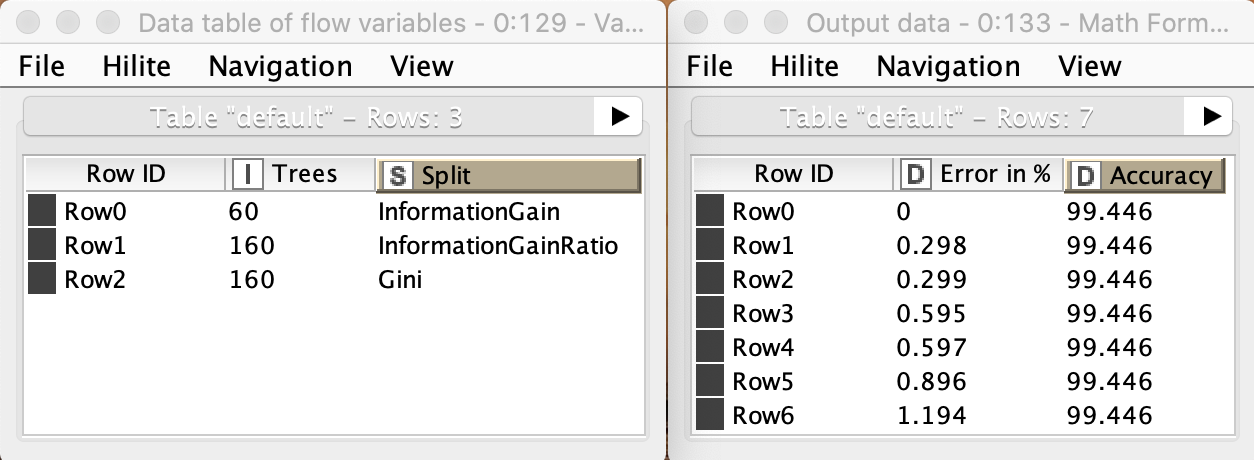
\includegraphics[width=15cm]{melhores_params}
	\caption{Melhores parâmetros para construir o modelo.}
\end{figure}

Por fim, sabendo quais os melhores parâmetros, contruiu-se um novo modelo usando $100\%$ dos dados para o treinar.

\begin{figure}[H]
	\centering
	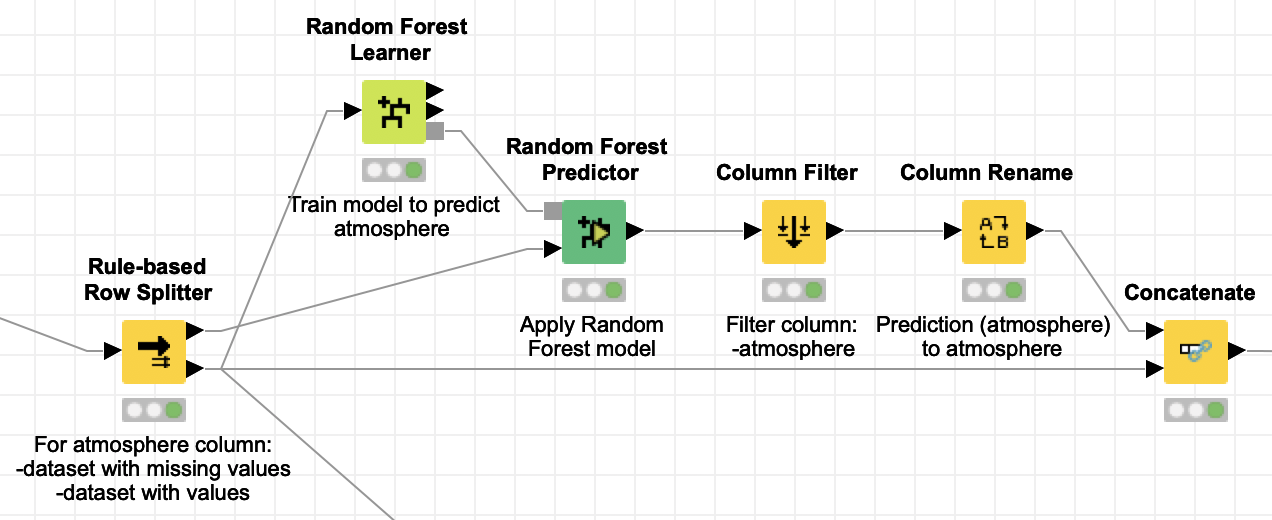
\includegraphics[width=15cm]{atmos}
	\caption{Previsão dos \textit{missing values} da \textit{feature atmosphere}.}
\end{figure}

Após feita a previsão dos \textit{missing values} para a \textit{feature atmosphere}, procedeu-se à previsão dos \textit{missing values} do atributo \textit{rain}, tendo-se utilizado o mesmo esquema para obter os melhores parâmetros, tendo-se obtido uma \textit{accuraccy} de cerca de $97,8\%$.

Para finalizar o tratamento de dados, no \textit{Knime}, recorrendo ao nodo \textit{Duplicate Row Filter}, eliminaram-se linhas repetidas e efetuou-se o \textit{Label Encoding} dos valores correspondentes às \textit{features}: \textit{Day of week (name)}, \textit{description}, \textit{incident\_category\_desc}, \textit{atmosphere} e \textit{rain}, uma vez que o objetivo é utilizar redes neuronais para prever o \textit{speed\_diff}, e estas apenas aceitam valores numéricos.

É de notar que, após feito todo este tratamento, existem colunas que apresentam \textit{missing values}. No entanto, estes \textit{missing values} ocorrem nas colunas correspondentes aos incidentes, porque não houve incidentes naquela hora, numa distância inferior a $0.5$ km. Estes \textit{missing values} foram substituídos por um valor \textit{default}, $-1$.

Por fim, observou-se que existiam dias com horas repetidas, devido ao facto de para uma mesma hora existir mais do que um incidente. Assim, para que isto não acontecesse, recorreu-se ao nodo \textit{GroupBy} para agrupar os incidentes, optando-se por ficar com o incidente que estava mais próximo da rua em estudo, ou seja, o incidente que apresentava na coluna \textit{Distance} o valor mais baixo.

\begin{figure}[H]
	\centering
	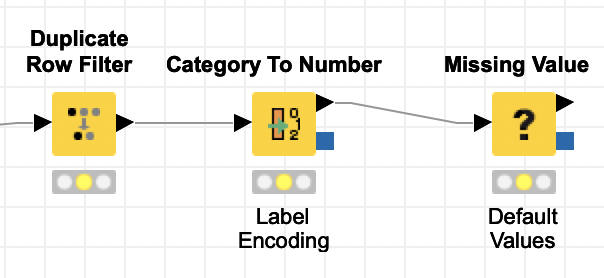
\includegraphics[width=8cm]{fim}
	\caption{Tratamento final.}
\end{figure}

Após feito este tratamento, recorrendo ao nodo \textit{Pie chart (local)} percebeu-se que o \textit{dataset} apresentava dias e horas em falta como, por exemplo, o mês de Março.

\begin{figure}[H]
	\centering
	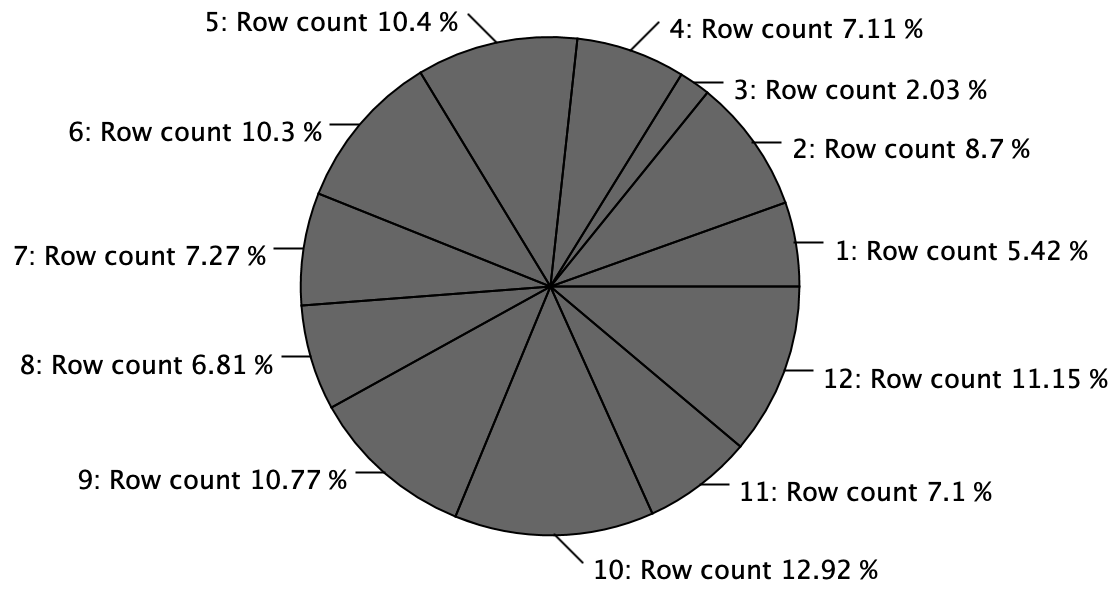
\includegraphics[width=8cm]{mes_dias}
	\caption{Dias em falta no \textit{dataset}.}
\end{figure}

\section{Problema}

O objetivo do trabalho consiste em utilizar Redes Neuronais para fazer previsão do fluxo de tráfego rodoviário. Tendo em conta os dados disponibilizados, o grupo optou por fazer a previsão da \textit{feature speed\_diff} de uma dada rua, baseando-se nos $3$ dias anteriores para prever o dia seguinte. Optou-se por fazer previsões para as ruas em separado, uma vez que se acredita que o fluxo de tráfego das ruas é distinto entre elas. Para isso, dividiu-se o \textit{dataset} original em $4$, sendo que cada \textit{dataset} correspondia a uma determinada rua.

Uma vez que se trata de um problema de séries temporais, optou-se por implementar um modelo \textit{multistep} e \textit{multivariate} que utiliza \textit{LSTM}'s.

\subsection{Resolução do Problema}

Para resolver este problema era então necessário perceber quais os dias que estavam incompletos, ou seja, quais os dias que não tinham as $24$ horas preenchidas, procedendo-se à eliminação destes, com o intuito de se ter um \textit{dataset} sem "buracos". Para isso, implementou-se o seguinte algoritmo:

\begin{lstlisting}[language=Python]
i=0
for i in range(1,13):
	for j in range(1,32):
	L=df[(df['Month (number)']==i)&(df['Day of month']==j)].dropna()
	L1=L[['Month (number)','Day of month','Hour','road_num']]
	L1 = L1.drop_duplicates()
	indexNames = df[(df['Month (number)']==i)&(df['Day of month']==j)].index
	if len(L1)<24:
	try:
		df.drop(indexNames, inplace=True)
	except:
		pass
\end{lstlisting}

Note-se que se verificou que nos dias em que havia horas em falta, normalmente o número de horas em falta era elevado, não se justificando a reconstrução dessas horas, recorrendo a métodos matemáticos, pelo que se optou por eliminar esses dias.

Visto que no final do capítulo \ref{section:falta} verificámos que existiam dias em falta e como se pretende que sejam dados ao modelo, como \textit{input}, $3$ dias para prever o próximo, quer garantir-se que, de facto, esses $4$ dias são seguidos, ou seja, que os $3$ dias dados como \textit{input} mais o dia a prever sejam seguidos, evitando que ocorram situações em que o primeiro dia seja, por exemplo, $16$ de Janeiro e o dia a prever seja $30$ de Janeiro.

Assim, para ter a certeza que se treina o modelo com dias consecutivos, percorreu-se o \textit{dataset} construindo blocos de $4$ dias, para verificar se estes $4$ dias são seguidos, calcula-se a diferença entre o último dia do bloco e o primeiro e verifica-se se é $4$. Note-se, no entanto, que se para um dado bloco tivermos dias de meses distintos, esta diferença é negativa, sendo este problema corrigido dependendo do mês em causa.

Antes de se aplicar o seguinte algoritmo, ordenou-se o \textit{dataset} por mês, dia e hora.

\begin{lstlisting}[language=Python]
n_future = 24 # next 24 hours speed diff forecast
n_past = 24*3 # Past 3 days

x_train = []
y_train = []
label = df_1['speed_diff']

for i in range(0,len(df_1)-n_past-n_future+1):
	dias = df_1.iloc[i : i + n_past+24]
	mes = dias.iloc[0]['Month (number)']
	dia_1 = dias.iloc[0]['Day of month']
	dia_4 = dias.iloc[24*3+1]['Day of month']
	if (mes == 4 or mes == 6 or mes == 9 or mes == 11) and (dia_4 - dia_1 == 3 or dia_4 - dia_1 == -29):
		x_train.append(df_1.iloc[i : i + n_past])
		y_train.append(label.iloc[i + n_past : i + n_past + n_future ])
	elif (mes == 1 or mes == 3 or mes == 5 or mes == 7 or mes == 8 or mes == 10 or mes == 12) and (dia_4 - dia_1 == 3 or dia_4 - dia_1 == -28):
		x_train.append(df_1.iloc[i : i + n_past])
		y_train.append(label.iloc[i + n_past : i + n_past + n_future ])
	elif mes == 2 and (dia_4 - dia_1 == 3 or dia_4 - dia_1 == -26):
		x_train.append(df_1.iloc[i : i + n_past])
		y_train.append(label.iloc[i + n_past : i + n_past + n_future ])
\end{lstlisting}

Sabendo-se que cada \textit{input} é constituído por $3$ dias seguidos, com as $24$ horas completas e, portanto, as colunas \textit{Month (number)}, \textit{Day of month} e \textit{Hour} já não são relevantes, tendo-se feito a remoção das mesmas. Além disso, removeram-se as colunas \textit{Day of week (name)}, \textit{incident\_category\_desc} e \textit{Distance}. Esta última foi removida, uma vez que apenas serviu para saber quais os incidentes que deviam permanecer no \textit{dataset}.

Após feito todo o tratamento acima mencionado, o \textit{dataset} está pronto para ser aplicado a uma rede que permita prever a \textit{feature speed\_diff}.

\section{Modelo}

O problema que se pretende resolver é um problema de séries temporais, como já foi anteriormente referido. Deste modo, para prever a \textit{feature speed\_diff} optou-se por construir um modelo \textit{multistep} e \textit{multivariate} que utiliza \textit{LSTM}'s.

Tendo em conta que o objetivo é utilizar $3$ dias para prever as $24$ horas seguintes, utilizando $11$ \textit{features}, definiu-se como $input_shape = (24*3,11)$.

Antes de se começar a treinar o modelo procedeu-se à normalização dos dados:

\begin{lstlisting}[language=Python]
# Features normalization
scalers=[]
for i in range(11):
sc = MinMaxScaler(feature_range=(0,1))
x_train[:,i] = sc.fit_transform(x_train[:,i])
x_test[:,i] = sc.fit_transform(x_test[:,i])
scalers.append(sc)

# Labels normalization
sc1 = MinMaxScaler(feature_range=(0,1))
y_train = sc1.fit_transform(y_train)
y_test_n = sc1.fit_transform(y_test)
\end{lstlisting}

Uma vez que os dados estavam normalizados no intervalo $[0,1]$ recorreu-se à função de ativação \textit{sigmoid}.

Relativamente às métricas utilizadas, utilizou-se como \textit{loss} o \textit{mean square error} e como métrica o \textit{root mean square error}. Estas foram as métricas escolhidas, uma vez que o  objetivo era penalizar erros grandes, e estas são as melhores métricas para o fazer.

Assim, recorrendo a técnicas de intuição e experimentação construiu-se o seguinte modelo:

\begin{lstlisting}[language=Python]
model = Sequential()
model.add(CuDNNLSTM(units=24*3, return_sequences=True, input_shape = (24*3,11) ) )
model.add(Dropout(0.2))
model.add(CuDNNLSTM(24*3 , return_sequences=True))
model.add(Dropout(0.2))
model.add(CuDNNLSTM(24*3, return_sequences=True))
model.add(Dropout(0.2))
model.add(CuDNNLSTM(24*2))
model.add(Dropout(0.2))
model.add(Dense(24,activation='sigmoid'))
model.compile(optimizer='adam', loss='mean_squared_error',metrics=rmse)
checkpointer = ModelCheckpoint(filepath="best_weights.hdf5", monitor = 'val_loss', verbose=1, save_best_only=True)
callback = tf.keras.callbacks.EarlyStopping(monitor='loss', patience=30)
history=model.fit(x_train, y_train, validation_data=(x_test, y_test_n), epochs=1000, callbacks=[callback, checkpointer])
\end{lstlisting}

Note-se que se recorreram a dois \textit{callbacks}: um para garantir que se guardava o melhor modelo, que seria porteriormente usado para fazer previsões, e outro que permitia que o treino parasse, quando não houvesse uma melhor do valor de \textit{loss} durante $30$ épocas seguidas.

\subsection{Avaliação do comportamento do modelo}

Após construído o modelo, procedeu-se a um conjunto de testes, utilizando $200$ dados de teste, com o intuito de ser possível avaliar o comportamento do mesmo.

Primeiro determinou-se, para os $200$ dados de teste, o número de ocorrências de cada dia da semana. Para se perceber se o comportamento do modelo era o esperado procedeu-se à utilização de duas métricas de erro, a média dos erros e a diferença absoluta, com a seguinte expressão, respetivamente:

\begin{center}
	\textit{average\_diff }=$\dfrac{\sum_{i}|\hat{y_i}-y_i|}{24}$, onde $i=0,..,23$\\
	\vspace{0.5cm}
\textit{max\_diff}=$\max{|\hat{y_i}-y_i|}$, onde $i=0,..,23$\\
\end{center}

Ambas as métricas de erro parecem ser úteis para perceber o comportamento do modelo. No entanto, a métrica \textit{max\_diff} apresenta melhores resultados para exemplos específicos. Considere-se um exemplo em que temos $23$ valores a $0$ e outro apresenta um speed\_diff de $15$ e, na previsão, o modelo acerta os $23$ casos em que é o valor era $0$, mas no caso em que o valor real era $15$ o valor previsto foi $9$. Então, neste caso, tem-se que {average\_diff }$=0.25$, o que nos dá um valor de erro baixo, induzindo-nos em erro ao acharmos que os valores previstos eram bons, o que não acontece, uma vez que o único valor que era difícil de prever o modelo erra por uma diferença de $6$ km. Por outro lado, a métrica \textit{max\_diff} diz-nos que o erro é $6$, o que permite concluir que o modelo não fez uma boa previsão para este exemplo.

\subsubsection{Rua 1}

Começou-se por treinar o modelo com $5045$ dados da rua $1$, e fazer a previsão para essa mesma rua. 

\begin{figure}[H]
	\centering
	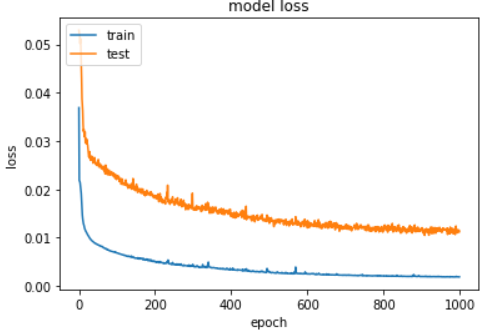
\includegraphics[width=10cm]{resultados/curvas_aprend_1.png}
	\caption{Curvas de aprendizagem.}
	\label{figure:curvas_aprend_1}
\end{figure}

Observando a Figura \ref{figure:curvas_aprend_1}, conclui-se que o modelo criado apresenta \textit{underfitting}, uma vez que as curvas de aprendizagem são distintas uma da outra. Pode ainda referir-se que, apesar de existir \textit{underfitting}, é provável que com o aumento do número de épocas não se observe uma convergência das curvas, uma vez que se verifica que ambas as curvas parecem ter estagnado, o que pode evidenciar que o modelo não está a aprender.

\begin{figure}[H]
	\centering
	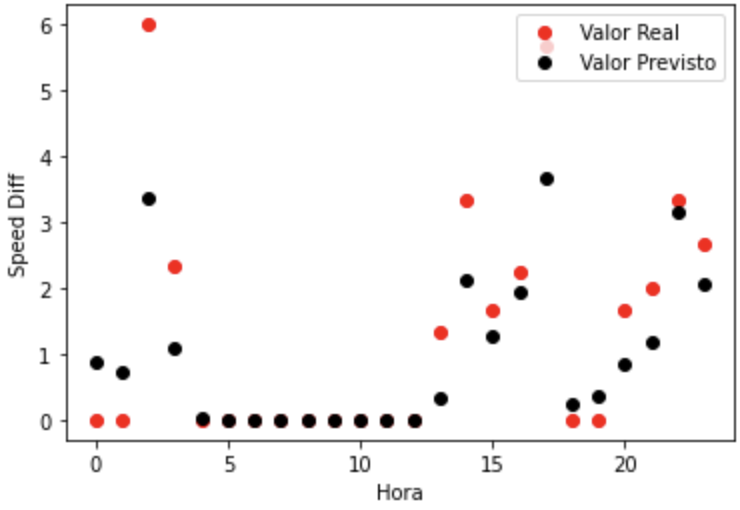
\includegraphics[width=10cm]{resultados/real_prev_1.png}
	\caption{Valores reais vs previstos, durante 24 horas, para um dia aleatório.}
	\label{figure:real_prev_1}
\end{figure}

\begin{table}[H]
	\centering
	\begin{tabular}{||c||c|c||}
		\hline\hline
		Hora & Real&Previsto\\
		\hline\hline
		0 & 0
		&0.88 \\
		\hline
		1  &
		0 & 0.73\\
		\hline
		2 & 6 & 	3.37\\
		\hline
		3  & 
		2.33
		&1.10 \\
		\hline
		4 & 
		0 & 0.023\\
		\hline
		5  & 
		0 &0.00017 \\
		\hline
		6 & 
		0
		& 
		0.00014
		\\
		\hline
		7 & 0
		
		&0.012 \\
		\hline
		8  &0
		&0.00011 \\
		\hline
		9 &  0& 0.00021	\\
		\hline
		10 & 0
		
		& 7.70e-05\\
		\hline
		11  &0
		& 1.90e-06\\
		\hline
		12 &0  & 0.00088	\\
		\hline
		13  & 
		1.33
		&0.32 \\
		\hline
		14 & 
		3.33 &2.13\\
		\hline
		15  & 1.67
		& 1.26\\
		\hline
		16 & 
		2.25
		& 
		1.95
		\\
		\hline
		17 & 
		5.67
		& 3.66\\
		\hline
		18  &
		0 &0.25 \\
		\hline
		19 &  0& 0.37	\\
		\hline
		20 & 
		1.67
		&0.86 \\
		\hline
		21  &
		2 & 1.19\\
		\hline
		22 &  3.33& 3.15	\\
		\hline
		23  & 
		2.67 
		&2.05\\
		\hline\hline
	\end{tabular}
\end{table}

A Figura \ref{figure:real_prev_1} e a tabela permitem comparar o valor previsto com o valor real, durante um período de $24$ horas. Ora, através da análise do gráfico, observa-se que não existe uma grande discrepância entre o valor real e o valor previsto. Pelo que se pode considerar que, para este caso, o modelo construído faz boas previsões. É de notar que, neste caso, os valores previstos são mais distintos dos valores reais às $3$ e $4$ da manhã, sendo normal que o modelo erre nestas horas, uma vez que não é comum que o valor do \textit{speed\_diff} seja mais elevado nestas, ou seja, pode inferir-se que este dia não representa os dias comuns.


Por fim, faça-se uma análise dos erros obtidos. Após calculados os diferentes valores do erro, obtiveram-se os seguinte resultados:

\begin{table}[H]
\centering
\begin{tabular}{||c||c|c|c||}
	\hline\hline
	 & Número de Ocurrências & \textit{Average Diff} & \textit{Max Diff} \\
	\hline\hline
	Segunda-Feira & 29&
	0.45
 & 2.69\\
	\hline
	 Terça-Feira  &32&
	0.67
 & 3.34\\
	\hline
	 Quarta-Feira & 21&
	0.73
 & 3.54
 \\
	\hline
	 Quinta-Feira  & 28&
	0.87
 & 3.57
   \\
	\hline
	 Sexta-Feira & 26&
	0.65 & 3.07
 \\
	\hline
	 Sábado  & 40&
	0.83 & 3.82   \\
	\hline
	 Domingo & 24&
0.36
 & 
2.91
 \\
	\hline\hline
\end{tabular}
\label{table:rua1}
\caption{Cálculo dos erros.}
\end{table}

Tendo em conta os gráficos e os resultados apresentados nas tabelas, pode concluir-se que o modelo prevê a \textit{feature speed\_diff} para esta rua com sucesso.

\subsubsection{Rua 2}

Considerando os dados de treino da rua $2$, treinou-se o modelo construído, obtendo-se os seguintes resultados.

\begin{figure}[H]
	\centering
	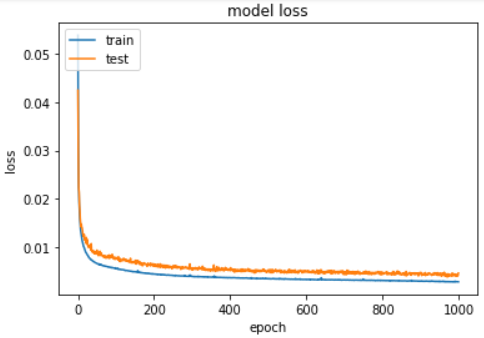
\includegraphics[width=10cm]{resultados/curvas_aprend_2.png}
	\caption{Curvas de aprendizagem.}
\end{figure}

Analisando o gráfico, observa-se que, em relação ao apresentado para a rua $1$, agora as curvas de aprendizagem estão mais próximas, sendo ainda possível observar-se que o modelo chegou ao seu limite de aprendizagem, uma vez que não se verifica um decréscimo da reta.

\begin{figure}[H]
	\centering
	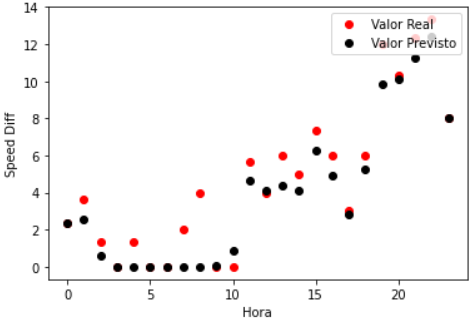
\includegraphics[width=10cm]{resultados/real_prev_2.png}
	\caption{Valores reais vs previstos, em 24 horas.}
\end{figure}

\begin{table}[H]
	\centering
	\begin{tabular}{||c||c|c||}
		\hline\hline
		Hora & Real&Previsto\\
		\hline\hline
		0 & 
		2.33
		&3.6011205 \\
		\hline
		1  &
		3.67 &3.05 \\
		\hline
		2 &  1.33& 0.98	\\
		\hline
		3  & 
		0
		&0.056 \\
		\hline
		4 & 1.33
		&0.00011 \\
		\hline
		5  & 
		0 &5.72e-07 \\
		\hline
		6 & 
		0
		& 
		
		1.04e-07 \\
		\hline
		7 & 
		2
		& 3.18e-08\\
		\hline
		8  &
		4 & 0.00016\\
		\hline
		9 &  0& 0.028	\\
		\hline
		10 & 
		0
		& 0.82\\
		\hline
		11  &
		5.67 & 5.46\\
		\hline
		12 & 4 & 4.28	\\
		\hline
		13  & 5.99
		
		&4.42 \\
		\hline
		14 & 
		5 &4.38 \\
		\hline
		15  & 7.33
		& 6.31 \\
		\hline
		16 & 
		5.99
		& 
		5.21
		\\
		\hline
		17 & 
		3.0
		& 2.84\\
		\hline
		18  &
		6.0 & 5.12\\
		\hline
		19 & 12.0 & 9.61	\\
		\hline
		20 & 
		10.33
		&10.15 \\
		\hline
		21  &
		12.33 &11.24 \\
		\hline
		22 & 13.33 & 12.63	\\
		\hline
		23  & 
		7.99
		& 8.48\\
		\hline\hline
	\end{tabular}
\end{table}

Analisando os resultados acima apresentados pode concluir-se, que para este exemplo, o modelo fez boas previsões. Estas conclusões são reforçadas pelos valores obtidos para as métricas de erro:

\begin{itemize}
	\item average\_diff
	\item max\_diff
\end{itemize}


Por fim, faça-se uma análise dos erros obtidos. Após calculados os diferentes valores do erro, obtiveram-se os seguinte resultados:

\begin{table}[H]
	\centering
	\begin{tabular}{||c||c|c|c||}
		\hline\hline
		& Número de Ocurrências & \textit{Average Diff} & \textit{Max Diff} \\
		\hline\hline
		 Segunda-Feira &29& 0.29& 1.38 \\
		\hline
		 Terça-Feira  &32&0.51 & 2.27\\
		\hline
		 Quarta-Feira&21 & 0.42& 1.70	\\
		\hline
		 Quinta-Feira&28  & 0.44& 1.78	\\
		\hline
		 Sexta-Feira &26& 0.48& 2.04  \\
		\hline
		 Sábado &40 & 0.43
 & 1.79\\
		\hline
		 Domingo & 24&
0.36 & 
1.80
\\
		\hline\hline
	\end{tabular}
	\label{table:rua2}
	\caption{Cálculo dos erros.}
\end{table}

Analisando os resultados dos erros observa-se que os valores obtidos são uniformes e semelhantes, ou seja, para esta rua, parece que o modelo prevê todos os dias com a mesma dificuldade, o que não se verificava no modelo da rua 1. Para o modelo da rua 1, verificou-se que este tinha mais dificuldade em prever Quintas-Feiras, do que Domingos.

\subsubsection{Rua 3}

Considerem-se agora os resultados obtidos pelo modelo treinado para a rua 3. Sabe-se que esta rua diz respeito à Rua do Caires, que corresponde a uma rua com bastante trânsito sendo, por isso, expectável grandes oscilações no valor da variável \textit{speed\_diff}, de uma hora para a outra.

\begin{figure}[H]
	\centering
	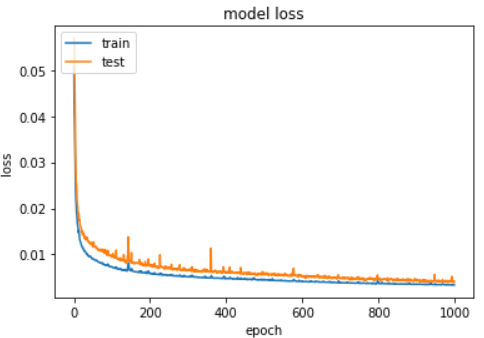
\includegraphics[width=10cm]{resultados/curvas_aprend_3.png}
	\caption{Curvas de aprendizagem.}
\end{figure}

À semelhança do que foi observado no exemplo anterior também aqui se verifica a convergência das curvas de aprendizagem.

\begin{figure}[H]
	\centering
	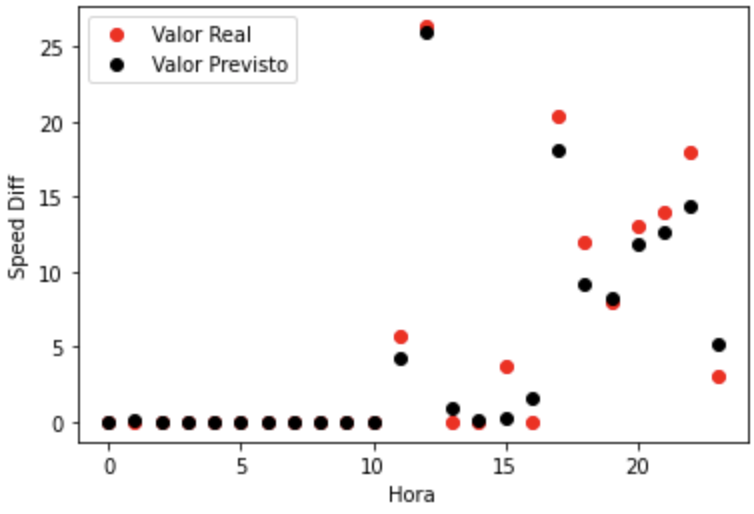
\includegraphics[width=10cm]{resultados/real_prev_3.png}
	\caption{Valores reais vs previstos, em 24 horas.}
\end{figure}

\begin{table}[H]
	\centering
	\begin{tabular}{||c||c|c||}
		\hline\hline
		Hora & Real&Previsto\\
		\hline\hline
		0 & 
0
 & 0.032280684 \\
		\hline
		1  &
0 & 0.06226761\\
		\hline
		2 & 0 & 0.0001824899	\\
		\hline
		3  & 
0
 & 0.002977331\\
		\hline
		4 & 0
 &0.038694322 \\
		\hline
		5  & 0
 &8.884608e-05 \\
		\hline
		6 & 0

 & 

7.37009e-05 \\
		\hline
		7 & 
0
 & 0.00014307268\\
		\hline
		8  &
0 & 1.6951117e-05\\
		\hline
		9 &  0& 0.0026792889	\\
		\hline
		10 & 

0 &0.009467335 \\
		\hline
		11  &
5.67 & 4.2219253\\
		\hline
		12 & 26.33 & 26.00911	\\
		\hline
		13  & 
0
 &0.9039111 \\
		\hline
		14 & 0
 &0.08721095 \\
		\hline
		15  & 
3.67 & 0.22982505\\
		\hline
		16 & 

0 & 
1.524076
 \\
		\hline
		17 & 
20.33
 & 18.167295 \\
		\hline
		18  &
12 & 9.12594 \\
		\hline
		19 & 7.99 & 8.301455	\\
		\hline
		20 & 
13
 &11.784495 \\
		\hline
		21  &
14 &12.6543255 \\
		\hline
		22 & 18 & 14.313829	\\
		\hline
		23  & 3

 & 5.1567326\\
		\hline\hline
	\end{tabular}
\end{table}

Note-se que à hora $12$ o \textit{speed\_diff} real era de $26.33$ e o modelo fez uma previsão de $26.00$, à semelhança do que aconteceu para a hora $17$, realçando o excelente desempenho do modelo ao prever este dia.

Por fim, faça-se uma análise dos erros obtidos. Após calculados os diferentes valores do erro, obtiveram-se os seguinte resultados:

\begin{table}[H]
	\centering
	\begin{tabular}{||c||c|c||}
		\hline\hline
		& \textit{Average Diff} & \textit{Max Diff} \\
		\hline\hline
		29 Segundas & 
1.1104795417657065
 & 5.096033663632976\\
		\hline
		32 Terças  &

1.264305124666961 & 5.205189819066919 \\
		\hline
		21 Quartas & 
1.1223343328243598
 & 4.69481890565819 \\
		\hline
		28 Quintas  & 
1.340759207220143
 & 5.520887696665271\\
		\hline
		26 Sextas & 1.0976789264484141
 & 4.579785451503434\\
		\hline
		40 Sábados  & 
1.2548639571139115& 4.768039370036238 \\
		\hline
		24 Domingos & 
0.5671839880583601
 & 
3.284548810598506 \\
		\hline\hline
	\end{tabular}
	\label{table:rua3}
	\caption{Cálculo dos erros.}
\end{table}

Apesar de se verificar, através do gráfico, que o modelo fez boas previsões, observa-se que os valores obtidos para os erros são mais elevados neste caso do que no caso dos modelos apresentados para as ruas $1$ e $2$. No entanto, basta olhar para o exemplo apresentado para verificar que esta rua apresenta valores para o \textit{speed\_diff} bastante elevados. De facto, para o exemplo apresentado o valor máximo para o \textit{speed\_diff} é de $26.33$km/h e, por exemplo, para o caso da rua $1$, o valor máximo do \textit{speed\_diff} é $5.67$ km/k. Assim, é importante notar que o modelo da rua $3$ tem que prever valores muito mais elevados do que o da rua $1$. Ou seja, dados estes valores pode dizer-se que errar $1$ km/h na rua $3$ pode ser considerado um erro menor do que errar $0.5$ km na rua $1$, concluindo-se, assim que, embora os erros apresentados nesta tabela sejam mais elevados, o nosso espírito crítico, leva-nos a concluir que o modelo da rua $3$ até pode ser considerado melhor que o da rua $1$.

\subsubsection{Rua 4}

A presente secção pretende analisar os resultados obtidos com o modelo treinado para a rua $4$. Note-se que, à semelhança da rua $3$, esta é uma rua com bastante trânsito, sendo expectável obterem-se resultados semelhantes aos apresentados para essa rua.

Apresentam-se, de seguida, os valores obtidos pelo modelo treinado com os dados da rua $4$. 

\begin{figure}[H]
	\centering
	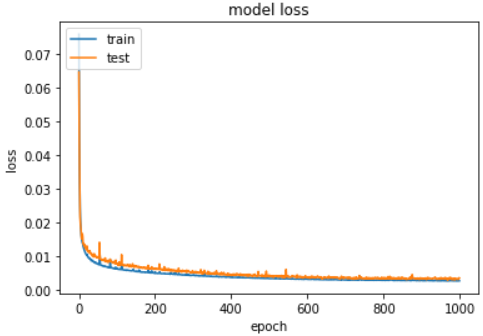
\includegraphics[width=10cm]{resultados/curvas_aprend_4.png}
	\caption{Curvas de aprendizagem.}
\end{figure}

Tal como observado para os gráficos das curvas de aprendizagem dos modelos das ruas $2$ e $3$, também para o modelo obtido para a rua $4$ se verifica que as curvas de aprendizagem estão a convergir.

\begin{figure}[H]
	\centering
	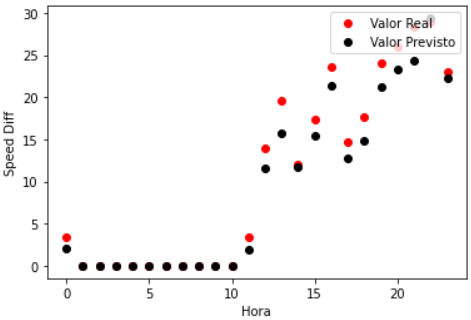
\includegraphics[width=10cm]{resultados/real_prev_4.png}
	\caption{Valores reais vs previstos, em 24 horas.}
\end{figure}

\begin{table}[H]
	\centering
	\begin{tabular}{||c||c|c||}
		\hline\hline
		Hora & Real&Previsto\\
		\hline\hline
		0 & 
3.33
 & 1.6831238\\
		\hline
		1  &
0 &0.0036463984 \\
		\hline
		2 & 0 & 	3.9301664e-09\\
		\hline
		3  & 0

 &  6.119647e-05\\
		\hline
		4 & 0
 &6.241123e-10 \\
		\hline
		5  &0 
 &2.987104e-06 \\
		\hline
		6 & 0

 & 

2.3474257e-05 \\
		\hline
		7 & 0

 & 0.00030335836\\
		\hline
		8  &0
 & 7.2902294e-05\\
		\hline
		9 & 0 &  2.5659345e-05	\\
		\hline
		10 & 
0
 & 0.022530494 \\
		\hline
		11  &
3.33 &3.0792594 \\
		\hline
		12 & 14 & 13.116628	\\
		\hline
		13  & 
19.67 
 &  15.995314\\
		\hline
		14 & 
 12.0 &  13.002526\\
		\hline
		15  & 17.33
 & 17.276192\\
		\hline
		16 & 
23.67
 & 21.827679

 \\
		\hline
		17 & 
14.67
 &13.331219 \\
		\hline
		18  &
 17.674& 16.39099\\
		\hline
		19 & 24 & 	22.018396\\
		\hline
		20 & 
26
 & 24.598763 \\
		\hline
		21  &
 28.33& 25.148285\\
		\hline
		22 & 29 & 29.302673	\\
		\hline
		23  & 
23
 & 21.183737\\
		\hline\hline
	\end{tabular}
\end{table}

Observando os resultados apresentados, tiram-se conclusões semelhantes às obtidas para o exemplo apresentado para a rua $3$.

Por fim, faça-se uma análise dos erros obtidos. Após calculados os diferentes valores do erro, obtiveram-se os seguinte resultados:

\begin{table}[H]
	\centering
	\begin{tabular}{||c||c|c||}
		\hline\hline
		& \textit{Average Diff} & \textit{Max Diff} \\
		\hline\hline
		29 Segundas & 
0.6434349814782563
 & 4.357169496163079\\
		\hline
		32 Terças  &
1.0732532610132068
 & 5.173105200712162 \\
		\hline
		21 Quartas & 
0.9179087441886314
 & 5.071644801119003 \\
		\hline
		28 Quintas  & 
1.1919938745260334
 & 5.7381584813503155 \\
		\hline
		26 Sextas & 0.91356394178488
 & 5.536007864537613 \\
		\hline
		40 Sábados  & 0.9611405798139803
& 4.2988463422039525 \\
		\hline
		24 Domingos & 
0.4436569034521404
 & 4.482812049263807
 \\
		\hline\hline
	\end{tabular}
	\label{table:rua4}
	\caption{Cálculo dos erros.}
\end{table}

Apesar destas ruas serem ruas com muito trânsito é de notar que, a rua 4 apresenta valores de erro mais baixos do que os da rua anterior, isto pode ter em conta o facto de que a rua 3 em certos meses, por exemplo, Junho, Julho, Agosto, quando não há período escolar, esta apresenta um valor de trânsito muita mais baixo, o que faz com que o nosso dataset apresente valores de speed diff menores neste período. Ou seja, ao treinar o modelo com estes dados, conjetura-se que o modelo criado possa não ser tão preciso.Isto para concluir que a rua $4$, sendo uma rua que apresenta o mesmo fluxo de trânsito durante um ano inteiro, uma das razões possíveis para os erros darem mais baixo para esta rua é o facto supramencionado.

\section{Extra}

O presente capítulo pretende analisar o comportamento dos modelos obtidos para as diferentes ruas, testando-os para outras ruas, e analisar o comportamento do modelo treinado com o \textit{dataset} no qual não foram incluído os incidentes.

\subsection{\textit{Dataset} sem incidentes}

Este subcapítulo pretende analisar o comportamento do modelo treinado com o \textit{dataset} sem incidentes, para a rua $2$, utilizando $8$ \textit{features}.

\begin{figure}[H]
	\centering
	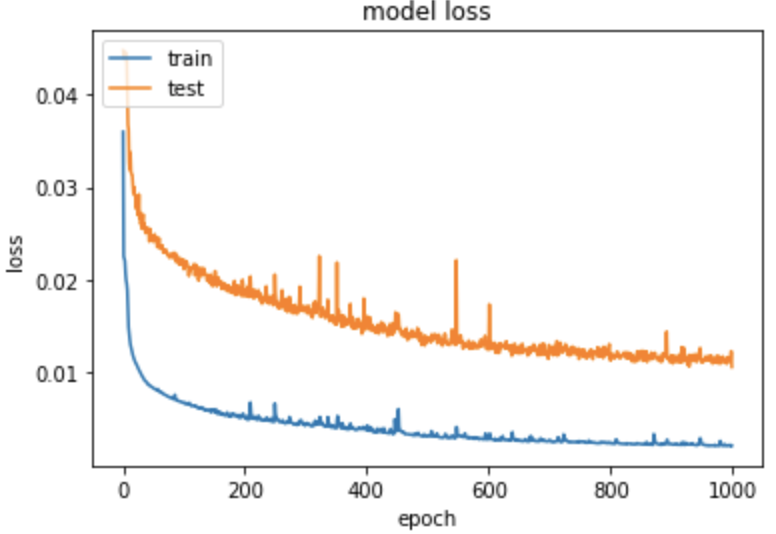
\includegraphics[width=10cm]{resultados/aprend_no_inc.png}
	\caption{Curvas de aprendizagem.}
\end{figure}

\begin{figure}[H]
	\centering
	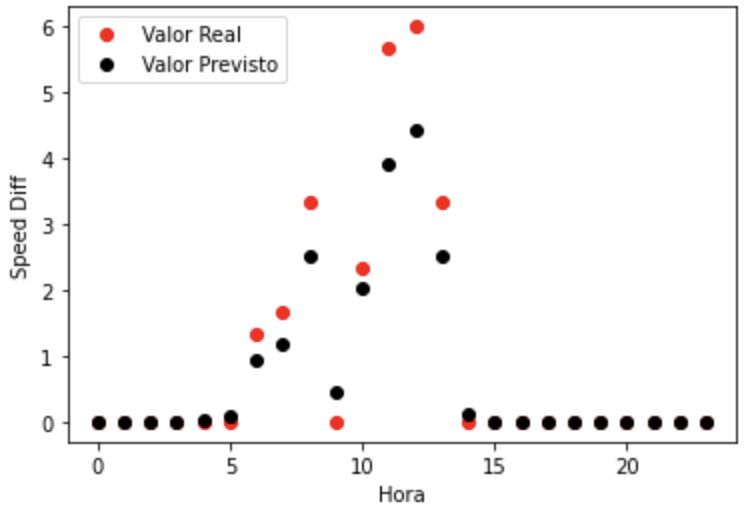
\includegraphics[width=10cm]{resultados/prev_real_no_inc.png}
	\caption{Valores reais vs previstos, em 24 horas.}
\end{figure}

\begin{table}[H]
	\centering
	\begin{tabular}{||c||c|c||}
		\hline\hline
		Hora & Real&Previsto\\
		\hline\hline
		0 & 
0
 & 6.9066814e-08 \\
		\hline
		1  &
0 & 2.5607434e-07\\
		\hline
		2 & 0 & 2.7351797e-07\\
		\hline
		3  & 0

 &2.0879885e-05 \\
		\hline
		4 & 0
 &0.01707314 \\
		\hline
		5  &0 
 &0.09949607 \\
		\hline
		6 & 1.33

 & 

0.9240082 \\
		\hline
		7 & 1.67

 & 1.1667032\\
		\hline
		8  &3.33
 & 2.5204258\\
		\hline
		9 & 0 &  0.45500085\\
		\hline
		10 & 
2.33
 &  2.0409627 \\
		\hline
		11  &
5.67 &3.920147 \\
		\hline
		12 & 6 &  4.414104\\
		\hline
		13  & 
3.33
 & 2.5295854 \\
		\hline
		14 & 
0  & 0.12146372\\
		\hline
		15  & 0
 &0.0020382823 \\
		\hline
		16 & 0
 & 
3.961704e-09 \\
		\hline
		17 & 
0
 & 6.731966e-08 \\
		\hline
		18  &
0 &1.2392364e-06 \\
		\hline
		19 &0  & 1.6075727e-07	\\
		\hline
		20 & 

0 & 1.254804e-06\\
		\hline
		21  &
0 & 1.0915311e-09\\
		\hline
		22 & 0 & 5.4359017e-12	\\
		\hline
		23  & 0

 & 4.7200618e-05 \\
		\hline\hline
	\end{tabular}
\end{table} 

Por fim, faça-se uma análise dos erros obtidos. Após calculados os diferentes valores do erro, obtiveram-se os seguinte resultados:

\begin{table}[H]
	\centering
	\begin{tabular}{||c||c|c||}
		\hline\hline
		& \textit{Average Diff} & \textit{Max Diff} \\
		\hline\hline
		29 Segundas & 
0.8580420333193335
 & 3.0794863584689107\\
		\hline
		32 Terças  &
0.8183510621136405& 3.096227680302678  \\
		\hline
		21 Quartas & 0.872193862194359
 & 2.8067537848154704 \\
		\hline
		28 Quintas  & 
0.8651441438734818
 & 2.96524466102997\\
		\hline
		26 Sextas & 1.04050743303996 & 3.0716054604671785 \\
		\hline
		40 Sábados  & 0.5317055662987664&2.3876666585233886  \\
		\hline
		24 Domingos & 0.5553113784184134
 & 2.172586509579598
 \\
		\hline\hline
	\end{tabular}
	\label{table:no_inc}
	\caption{Cálculo dos erros.}
\end{table}

Analisando os resultados apresentados na tabela e comparando-os com os obtidos no subcapítulo $4.1.2$, observa-se que estes são muito mais elevados, o que nos permite concluir que os dados relativos aos incidentes têm grande importância na previsão do \textit{speed\_diff}.

\subsection{Usar modelo da rua 2 para fazer previsões para a rua 1}

Decidiu-se testar o modelo da rua $2$ na rua $1$ uma vez que estas ruas são semelhantes. Note-se ainda que se optou por testar o comportamento do modelo treinado com a rua $2$, uma vez que este era o que apresentava melhores resultados.

Veja-se o comportamento do modelo treinado com dados da rua $2$, para fazer previsões para a rua $1$.

De seguida, apresenta-se, graficamente, os resultados obtidos, para um dia de teste:

\begin{figure}[H]
	\centering
	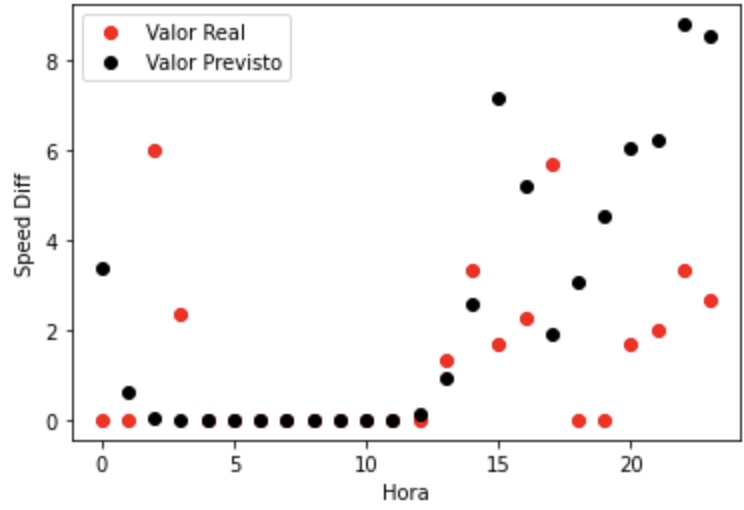
\includegraphics[width=10cm]{resultados/real_prev_mod2_rua1.png}
	\caption{Valores reais vs previstos, em 24 horas.}
\end{figure}

Analisando o gráfico, conclui-se que o modelo não se comporta de modo ótimo. Note-se que, nas horas $22$ e $23$ existe uma grande discrepância nos valores.

Relativamente aos erros obtidos, foram os seguintes:

\begin{table}[H]
	\centering
	\begin{tabular}{||c||c|c||}
		\hline\hline
		& \textit{Average Diff} & \textit{Max Diff} \\
		\hline\hline
		Segundas & 1.4970504526843698
		& 6.902452780405327 \\
		\hline
		Terças  &
		1.5817615829476248
		& 7.0771182393603675 \\
		\hline
		Quartas & 
		1.564599320078336 & 7.752798380280793	\\
		\hline
		Quintas  & 1.7489723562496609
		& 6.787156304928169	\\
		\hline
		Sextas & 
		1.8400726700992243 & 7.6605935197642 \\
		\hline
		Sábados  & 1.7762016329303
		& 7.453315566827695 \\
		\hline
		Domingos & 
		1.766229661484953 & 
		7.906649859769938
		\\
		\hline\hline
	\end{tabular}
	\label{table:mod2_rua1}
	\caption{Cálculo dos erros.}
\end{table}

Por fim, analisando o valor obtido para os erros observa-se que estes são superiores aos obtidos quando se usou o modelo treinado com a rua $2$ para fazer a previsão da variável \textit{speed\_diff} para essa mesma rua.

\subsection{Usar modelo da rua 1 para fazer previsões para a rua 3}

O presente subcapítulo pretende

De seguida, apresenta-se, graficamente, os resultados obtidos, para o primeiro dia de teste:

\begin{figure}[H]
	\centering
	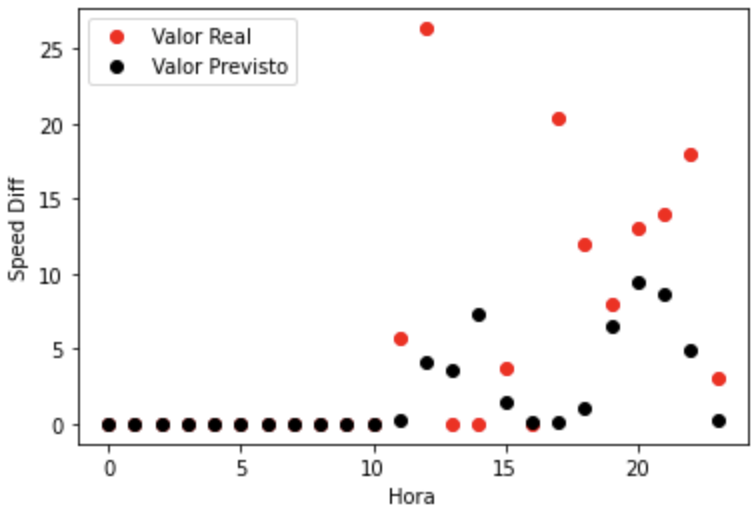
\includegraphics[width=10cm]{resultados/real_prev_mod1_rua3.png}
	\caption{Valores reais vs previstos, em 24 horas.}
\end{figure}

Relativamente aos erros obtidos, foram os seguintes:

\begin{table}[H]
	\centering
	\begin{tabular}{||c||c|c|c||}
		\hline\hline
		& Número de ocurrências &\textit{Average Diff} & \textit{Max Diff} \\
		\hline\hline
		 Segundas &29 & 4.97
		& 21.61 \\
		\hline
		 Terças  &32&
		4.51
		& 20.73\\
		\hline
		 Quartas & 21&4.85
		
		& 18.83	\\
		\hline
		 Quintas  & 28&
		4.64
		&	17.88\\
		\hline
		 Sextas & 26&
		4.00 & 15.85 \\
		\hline
		 Sábados  &40& 5.07
		& 21.99 \\
		\hline
		 Domingos & 24&
		3.64
		& 13.07
		
		\\
		\hline\hline
	\end{tabular}
	\label{table:mod1_rua3}
	\caption{Cálculo dos erros.}
\end{table}

Verificando os resultados, observam-se erros muito elevados. Isto deve-se ao facto do modelo prever valores de \textit{speed\_diff} baixos, uma vez que a rua $1$ apresenta um baixo fluxo de trânsito valores baixos para a \textit{speed\_diff}, e a rua $3$ ser uma rua com bastante trânsito e apresentar valores de \textit{speed\_diff} bastantes elevados.




\end{document}
